\documentclass{article}

\usepackage[dutch]{babel}
\usepackage[margin=3cm]{geometry}
\usepackage{graphicx}
\usepackage{float}
\usepackage{caption}
\usepackage{hyperref}
\usepackage{amsmath}
\usepackage{wrapfig}
\usepackage[parfill]{parskip}

% fonts
\usepackage[T1]{fontenc}
\usepackage{helvet}
\renewcommand{\familydefault}{\sfdefault}

\graphicspath{{img/}}
 
\newcommand{\bold}[1]{\textbf{#1}}

%Define the listing package
\usepackage{listings} %code highlighter
\usepackage{upquote}
\usepackage{color} %use color
\definecolor{mygreen}{rgb}{0,0.6,0}
\definecolor{mygray}{rgb}{0.5,0.5,0.5}
\definecolor{mymauve}{rgb}{0.58,0,0.82}

\begin{document}

\begin{titlepage}
    \author{Tuur Vanhoutte}
    \title{Security}
\end{titlepage}

\pagenumbering{gobble}
\maketitle
\newpage
\tableofcontents
\newpage

\pagenumbering{arabic}

\section{Security}

\subsection{Doel}
\begin{itemize}
    \item Security awareness  (bewustwording)
    \item Correcte nomenclatuur (communicatie)
    \item Advies over verantwoordelijkheden
    \item Inzien v/d consequenties v/h falen van security
    \item Situeren en herkennen van problemen
    \item Oplossingen correct implementeren
    \item Correcte methodieken toepassen
\end{itemize}

\subsection{Waarom?}

\begin{itemize}
    \item Niet iedereen heeft even goede bedoelingen
    \item Grote hoeveelheid mensen = veel potenti"ele slachtoffers (internet == iedereen zeer bereikbaar)
    \item Er is geen magische one-size-fits-all oplossing
    \item Verantwoordelijkheid van iedereen
    \item Tegenmaatregelen nemen
    \item Alert en voorzichtig zijn
\end{itemize}


\subsection{Tegenmaatregelen}
\begin{itemize}
    \item Zijn slechts nuttig indien ze effectief worden gebruikt
    \item Lijken vaak in de weg te zitten of lastig, maar zijn noodzakelijk
\end{itemize}

\subsection{Risico}

\begin{figure}[H]
    \centering
    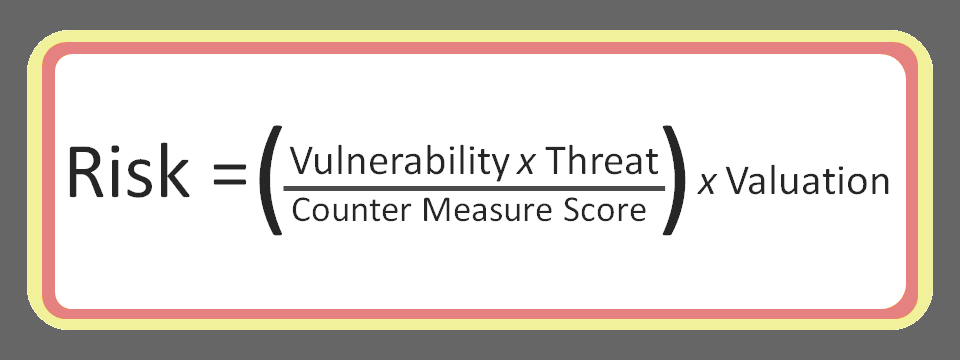
\includegraphics[width=0.4\textwidth]{risk.png}
    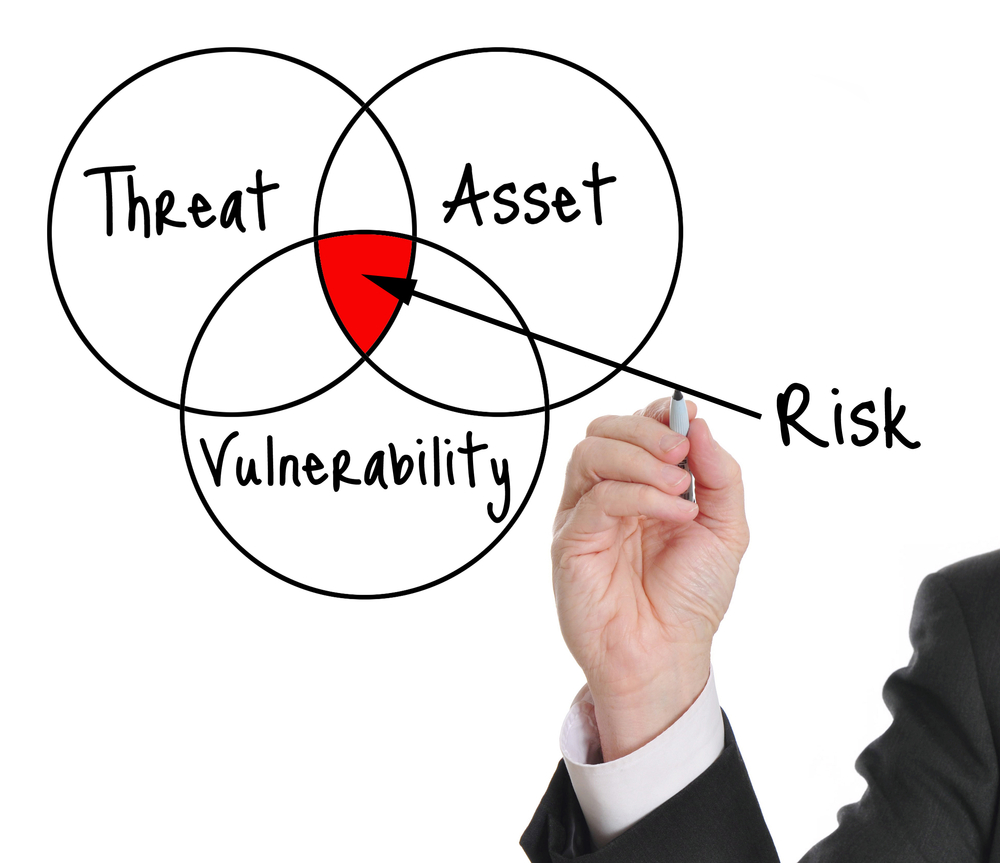
\includegraphics[width=0.25\textwidth]{01.png}
    \caption{Risico}
\end{figure}


\begin{itemize}
    \item De mate van bedreiging is niet beheersbaar
    \item De kwetsbaarheid is te reduceren door de implementatie van tegenmaatregelen
    \item Tegenmaatregelen reduceren kwetsbaarheid
    \item Bedrijfsimpact van het risico bepaalt de opportuniteit van de beveiligingsinvestering
    \item Bepalen van de financiële impact van een incident is uitermate bedrijfsspecifiek
\end{itemize}




\subsection{Theoretisch model}
\textcolor{red}{\bold{WORDT GEVRAAGD OP EXAMEN}}

\bold{CIA-model}

\begin{itemize}
    \item Confidentiality (Vertrouwelijkheid)
    \item Integrity (Integriteit)
    \item Availability (Beschikbaarheid)
\end{itemize}

\begin{figure}[H]
    \centering
    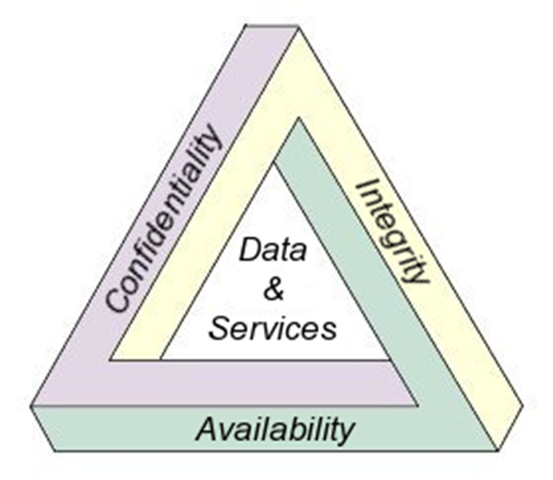
\includegraphics[width=0.3\textwidth]{cia-model.png}
    \caption{CIA-model}
\end{figure}

\bold{Vertrouwelijkheid}: gegevens kunnen \textit{enkel} door de juiste partijen worden geraadpleegd.

\bold{Integriteit}: gegevens zijn vaststaand en veranderen niet, tenzij de juiste, gemachtigde personen ze veranderen.

\bold{Beschikbaarheid}: de gegevens zijn beschikbaar en te bekijken door de juiste partijen, ongeacht aanvallen zoals DDOS-attacks.

\url{https://en.wikipedia.org/wiki/Information_security#Confidentiality}

\url{https://en.wikipedia.org/wiki/Information_security#Integrity}

\url{https://en.wikipedia.org/wiki/Information_security#Availability}

\subsubsection{Voorbeelden}

TODO

\subsection{Bedreiging vs kwetsbaarheid}
\bold{Bedreiging (threat)} = potenti"ele negatieve actie dat een ongewenste impact heeft op een computersysteem of applicatie.

\bold{Kwetsbaarheid (vulnerability)} = zwak punt in een computersysteem of applicatie die kan worden ge"exploiteerd. 

\subsubsection{Bedreigde doelen}
\begin{itemize}
    \item Infrastructuur
    \item Gegevens
    \item Operationaliteit
\end{itemize}

\begin{figure}[H]
    \centering
    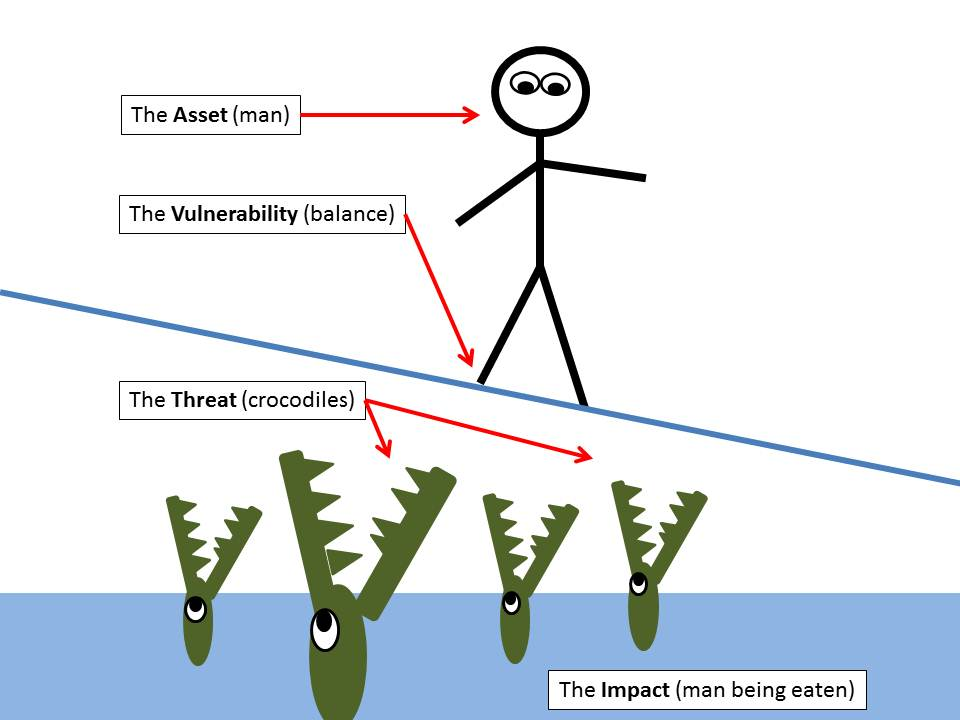
\includegraphics[width=0.5\textwidth]{crocodiles.jpg}
    \caption{}
\end{figure}

\section{Bedreigingen}

\begin{itemize}
    \item Vallen 1 of meerdere doelen aan
    \item Kunnen toevallig of kwaadwillig beraamd zijn
    \item Gaan uit van `agenten' (personen/organistaties) of gebeurtenissen
\end{itemize}

\subsection{Voorbeelden}

\begin{itemize}
    \item Phishing
    \item Smishing
    \item Vishing
    \item Money rules
    \item Malware
    \item Hardware uit onbetrouwbare bron
    \item Social engineering
    \item \dots
\end{itemize}

\subsection{Types}

\begin{itemize}
    \item Systeemfouten
    \item Gebeurtenissen
    \begin{itemize}
        \item Brand
        \item Stroomuitval
    \end{itemize}
    \item Intern
    \begin{itemize}
        \item Diefstal
        \item Wraak
    \end{itemize}
    \item Extern
    \begin{itemize}
        \item `Hackers'
        \item Spionage
    \end{itemize}
\end{itemize}

\subsection{Phishing}

\begin{itemize}
    \item Oplichting over email
    \item Vaak onwaarschijnlijk verhaal
    \item Vaak herkenbaar malifide links
    \item Soms bijzonder moeilijk herkenbaar
    \item Is de meest voorkomende vorm van fraude
    \item Is de meest uitgebuite kwetsbaarheid van een organisatie
    \item Zo veel mogelijk mensen bereiken, hopen dat een paar mensen toehappen.
\end{itemize}

\subsubsection{Geavanceerde vormen van phishing}

\begin{itemize}
    \item Spear phishing
    \begin{itemize}
        \item doelgerichter
        \item specifiek
        \item afzender spoofen naar iemand die het slachtoffer persoonlijk kent, slachtoffer aanspreken met echte naam
    \end{itemize}
    \item Double barrel attack
    \begin{itemize}
        \item Double barrel = tweeloopsgeweer
        \item Twee emails sturen: 1 heel duidelijk spam, de andere een reactie van de organisatie (bvb bank) die vraagt om op te letten voor phishing mails. 
        \item De tweede mail bevat vaak een link om je wachtwoord te veranderen $\Rightarrow$ link naar valse site
    \end{itemize}
\end{itemize}

\subsubsection{Andere vormen van phishing}

\begin{itemize}
    \item Bank card phishing
    \item CEO-Fraude
    \begin{itemize}
        \item Impersoneren van een CEO om in zijn/haar naam een actie te verrichten
        \item Bvb: leverancier contacteren om betaling op ander rekening nummer te storten
    \end{itemize}
    \item Factuurfraude
    \begin{itemize}
        \item Vroeger: een echte factuur uit een brievenbus nemen, rekeningnummer veranderen en opnieuw in de bus doen
        \item Tegenwoordig: valse facturen opsturen via email
    \end{itemize}
\end{itemize}

\subsubsection{Phishing herkennen}
\begin{itemize}
    \item Afzender controleren
    \item Taalgebruik
    \item Datum controleren: in het weekend moeilijker om om hulp te vragen aan de echte organisatie 
    \item Slachtoffer afschrikken met gerechtelijke stappen ondernemen
    \item Specifieren van extra informatie (bv: u heeft op maandag 01/02/2020 om 16:04 \textit{x} gedaan, daarom moet u nu \textit{y} betalen)
    \item Slachtoffer moet stappen ondernemen om de situatie niet nog erger te maken
    \item Gebruik van legitieme bedrijven om de transactie te voltooien (bv iTuneskaarten, Google Play kaarten, www.becharge.be)
\end{itemize}


\subsection{Smishing}
Oplichting via: \dots
\begin{itemize}
    \item SMS
    \item Whatsapp
    \item Facebook
    \item \dots
\end{itemize}

\subsection{Vishing}
= Voice Sollicitation 

\begin{itemize}
    \item Mensen bellen je op en maken je wijs dat ze u willen helpen om een probleem op te lossen
    \item Vaak pc overnemen met teamviewer en dergelijke
    \item Geld vragen om pc te `herstellen'
    \item Zie ook: refund scams, IRS scams, \dots
\end{itemize}

\subsection{Money mule}
= iemand die zijn/haar bankrekening laat misbruiken voor criminele activiteiten. 

\begin{itemize}
    \item De crimineel contacteert het slachtoffer met een jobaanbieding
    \item De job bestaat uit het overschrijven van bedragen via zijn/haar bankrekening
    \item Voor elke overschrijving 
\end{itemize}

\subsection{Malware}
= Software met als doel kwaad te berokkenen

\begin{itemize}
    \item Trojan
    \item Adware
    \item Virus / worm
    \item Ransomware
    \item Browser Malware
    \item Ook op smartphone
\end{itemize}

\subsection{Ransomware}
Maakt de data op je PC onbruikbaar tot je losgeld betaalt aan de criminelen.

\begin{itemize}
    \item `Kidnappen' van bestanden: bestanden openen niet langer mogelijk
    \item Poging tot innen van losgeld
    \item Vaak via phishing
    \item Enkel een backup van de gegevens kan voldoende beschermen
\end{itemize}

\subsubsection{Voorbeelden}

\begin{itemize}
    \item Wildfire\_locker
    \item Wannacry
    \item Cryptolocker
    \item Bad Rabbit
\end{itemize}

\subsection{Hardware uit onbetrouwbare bron}
\begin{itemize}
    \item USB Rubber ducky
    \begin{itemize}
        \item USB-stick die ergens gedropt wordt (= drop attack), het slachtoffer vindt de USB stick en stopt hem in zijn/haar computer (bvb uit nieuwsgierigheid).
        \item De USB stick werkt als een toetsenbord en typt een attack script op de pc van het slachtoffer
        \item Doel: volledige controle over PC, met bvb remote access (RAT = Remote Access Tool).
    \end{itemize}
\end{itemize}

\subsection{Vreemde netwerken}
\begin{itemize}
    \item Openbare netwerken kunnen worden afgeluisterd
    \item Verkeer op niet-vertrouwde netwerken kan worden omgeleid
\end{itemize}

\begin{figure}[H]
    \centering
    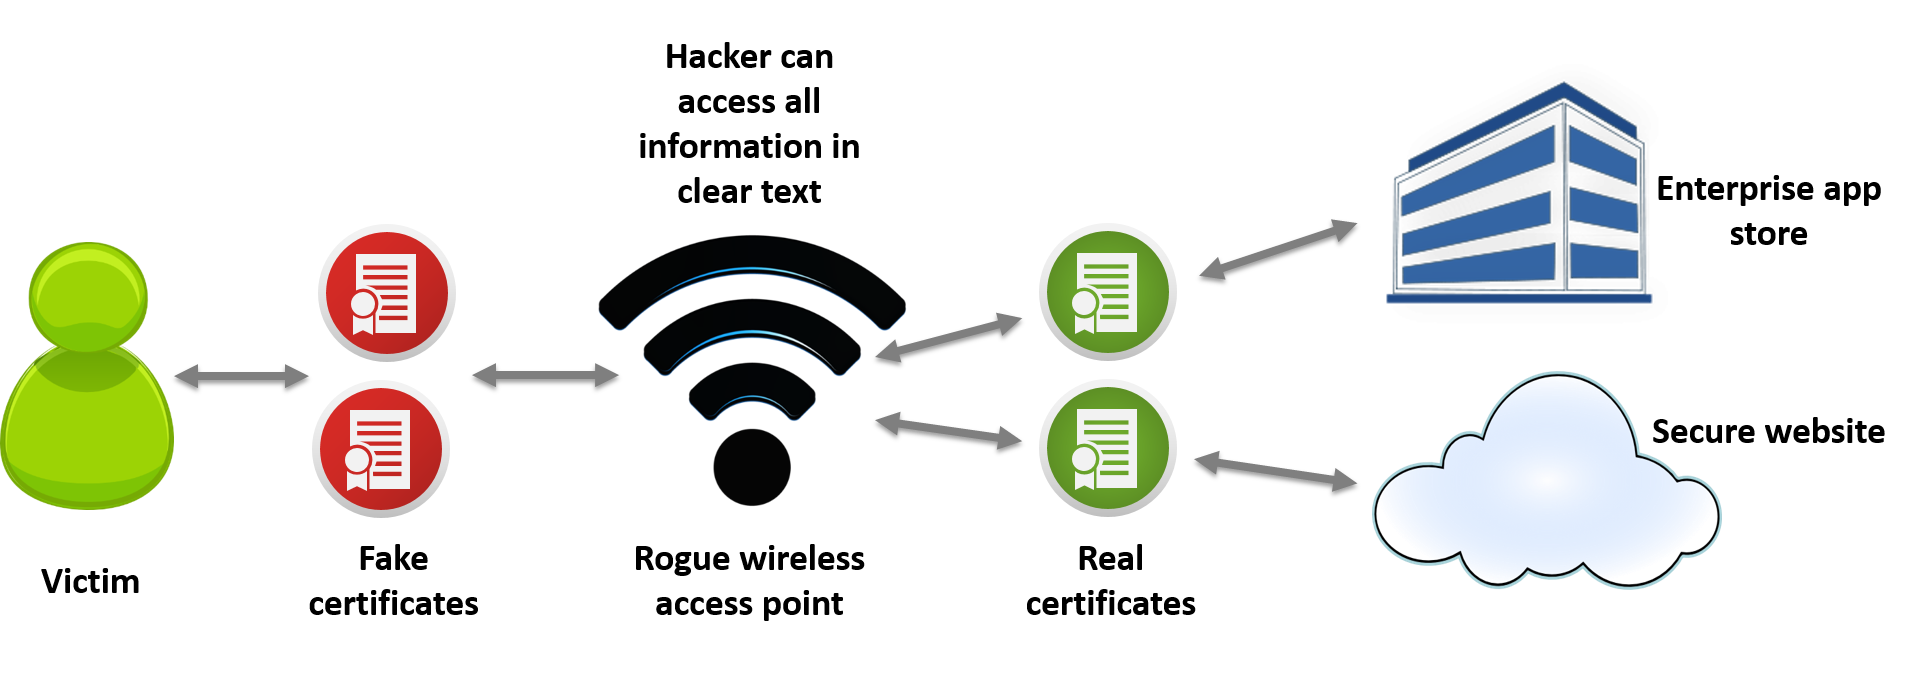
\includegraphics[width=0.5\textwidth]{vreemde-netwerken.png}
    \caption{Vreemde netwerken}
\end{figure}

\subsection{Social engineering}
Een techniek waarbij een crimineel een aanval op computersystemen tracht te ondernemen door de zwakste schakel in de computerbeveiliging, namelijk de mens, te kraken.


\subsection{Bedreigingen: `Agenten'}

\begin{itemize}
    \item Entiteiten waarvan de bedreiging uitgaat
    \item Zijn intern (=werknemers) of extern aan het bedrijf
    \item Kwetsbaarheid voor een agent wordt bepaald door zijn: 
    \begin{itemize}
        \item Toegangsniveau
        \item Kennis
        \item Motivatie
    \end{itemize}
\end{itemize}

\subsubsection{De ontslagen werknemer}
\begin{itemize}
    \item Heeft toegang (nog steeds?) tot de organisatie
    \item Heeft kennis over de werking van de organisatie
    \item Heeft een sterke negatieve motivatie
\end{itemize}

\subsubsection{De `hacker'}
De stereotiepe `hacker':
\begin{itemize}
    \item De blueprint opgevoerd door de media
    \item Is gebaseerd op reele figuren
    \item Vormt een rolmodel voor een bepaalde subcultuur
    \item Het woord `hacker' is vaak nietszeggend
    \item `Script kiddies', `Wannabees', `Crackers'
    \item Bedreiging groot door grote aantallen
    \item Hoofddeksels (hacker ethics):
    \begin{itemize}
        \item Black hat (=informatiecrimineel, voor persoonlijk gewin)
        \item White hat (`for the greater good', `etische hacker')
        \item Gray hat (iets tussen de twee)
    \end{itemize}
\end{itemize}

\bold{De `ethical' hacker}
= iemand die beveiligingen breekt om te tonen dat ze onveilig zijn

\begin{itemize}
    \item Goed of slecht voor security?
    \item Vb: security by obscurity (= niemand weet hoe het werkt dus het is veilig $\Rightarrow$ reeds vele malen slecht idee gebleken)
    \item Penetration testing (= verificatie van beveiliging, maar: mag niet ongevraagd, anders illegaal)
    \item Soms grijze zone
    \item Meldingsplicht? Welke wetgeving? 
    \item Responsible disclosure: firma inlichten ipv volledig internet
\end{itemize}

\subsection{Bedreigingen: gebeurtenissen}

\begin{itemize}
    \item Brand
    \item Stroomuitval
    \item Overstroming
    \item Diefstal
    \item Aanslag
\end{itemize}


\subsection{Threat intelligence}

\begin{itemize}
    \item `Know your enemy'
    \item Noodzakelijk om risico in te schatten
    \item Bijgevolg elementair om te beslissen over opportuniteit van \bold{tegenmaatregelen}
\end{itemize}

Real-time maps

\begin{itemize}
    \item \url{https://www.fireeye.com/cyber-map/threat-map.html}
    \item \url{http://cybermap.kaspersky.com/}
    \item \url{http://map.ipviking.com/}
\end{itemize}

\begin{figure}[H]
    \centering
    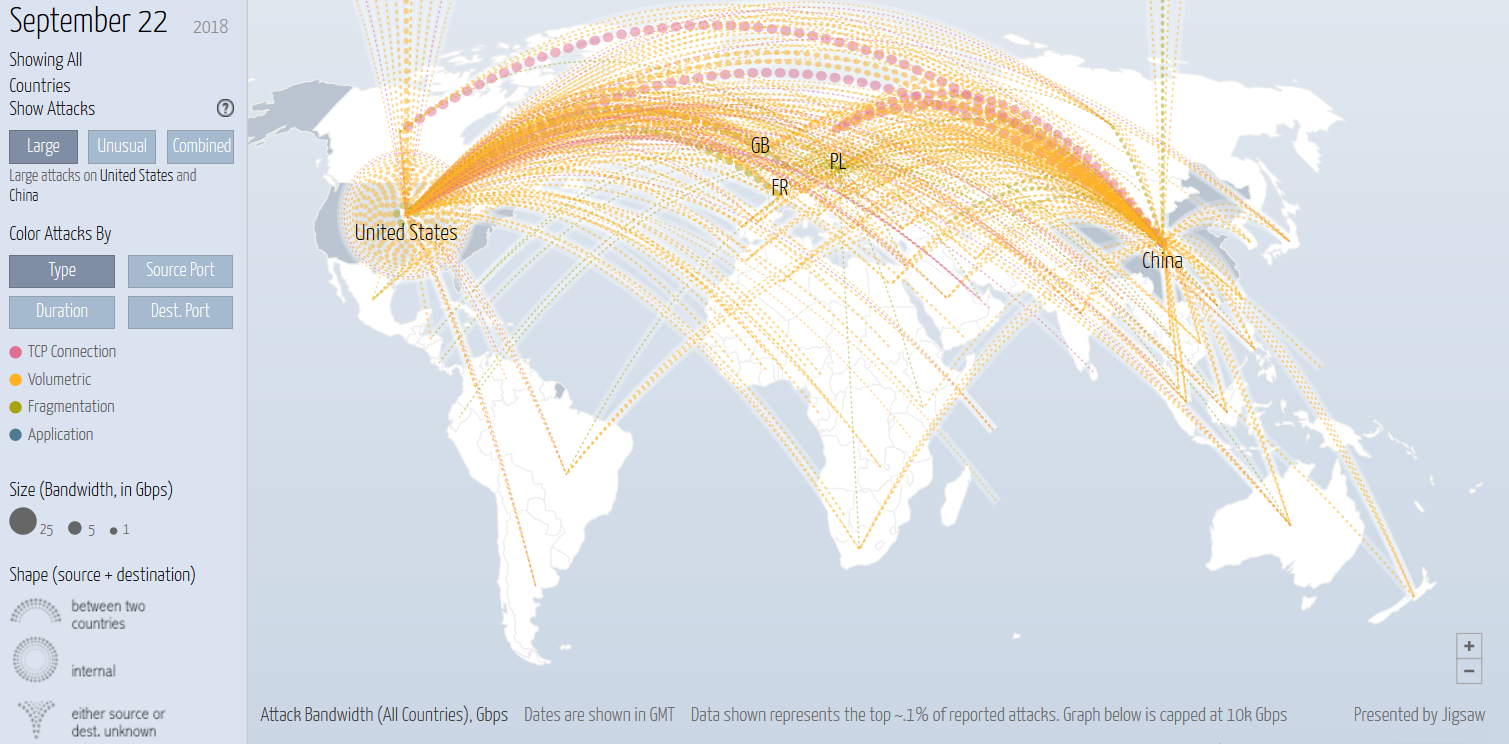
\includegraphics[width=0.8\textwidth]{threat-intelligence.png}
    \caption{Threat intelligence}
\end{figure}

\section{Beveiligen}

\subsection{Herhaling: kwetsbaarheden}

\begin{itemize}
    \item Software vulnerabilities
    \begin{itemize}
        \item Geen updates
        \item Foutief patch management
    \end{itemize}
    \item Interne toegang
    \begin{itemize}
        \item Misbruik machtigingen
        \item Wraak / ontslaan van werknemer
    \end{itemize}
    \item Extern bereikbare diensten
    \item Phishing / spear phishing
    \begin{itemize}
        \item The human factor
        \item Meest gebruikte entrypoint
        \item Email (SMTP) is niet geauthentiseerd
    \end{itemize}
\end{itemize}

\subsection{Shodan search engine demo}

\begin{itemize}
    \item \url{http://www.shodanhq.com}
    \item Zoekt naar geconnecteerde devices
    \item Webcams, videofoons, windturbines, waterkrachtcentrales, PLC's, \dots
\end{itemize}


\subsection{ICT security}
\begin{itemize}
    \item Is zeer complex
    \item Omvat erg veel, zeer diverse kennisdomeinen
    \item Wordt erg vaak over-gesimplificeerd
\end{itemize}

\subsubsection{Usability vs Security}
\bold{Extremen:}

\begin{itemize}
    \item Totale security is enkel mogelijk bij onbestaande usability
    \item Optimale usability is enkel mogelijk bij onbestaande security
\end{itemize}

"In any implementation of security controls all three factors:

\begin{enumerate}
    \item Security 
    \item Functionality
    \item Ease of Use
\end{enumerate}

are to be carefully considered; searching for the balanced trade-off for all stakeholders."

Een bruikbare infrastructuur kan nooit 100\% veilig zijn $\Rightarrow$ voorzichtig afwegen van alle parameters en belangen

\subsection{Tegenmaatregelen (mitigation)}

\begin{itemize}
    \item Corporate policy  - Training  - Awareness
    \item Coding practices
    \item Testing (Pentesting)
    \item Vulnerability management
    \item Backup
    \item Disaster recovery plan
    \item Fysieke Security
    \item Firewalls / IDS / IPS
\end{itemize}

\subsubsection{Defense in depth}
\begin{itemize}
    \item Layered security
    \item Strategie bij incident
    \item Plannen en documenteren
\end{itemize}

\begin{figure}[H]
    \centering
    
\includegraphics[width=0.5\textwidth]{layered-security.png}
    \caption{Layered security}
\end{figure}

\subsection{ICC / Belgian Cyber Security Guide}

\begin{itemize}
    \item Checklist
    \item Do's \& Dont's
    \item Gratis te downloaden: \url{http://iccbelgium.be/becybersecure/}
\end{itemize}



\end{document}